%!TEX root = ../thesis.tex
%*******************************************************************************
%****************************** Third Chapter **********************************
%*******************************************************************************
\chapter{Resultados y Discusión}\label{chap:result}

\begin{graybox}
\begin{itemize}
\item El principal resultado de este trabajo es la extensión \pgland{}, en la cual se ha colaborado en un importante porcentaje de funcionalidades (\textit{commits}).
\item Las métricas implementadas en forma de funciones se han validado sistemáticamente para asegurar que devuelven el resultado correcto.
\item Se ha desarrollado un caso de uso completo basado en la aplicación propuesta en la introducción (ver Figura \ref{fig:visorweb}) con el que se han obtenido resultados prometedores (\textit{usabilidad} y volumen).
\end{itemize}
\end{graybox}


En este capítulo se presentan los resultados de este trabajo siguiendo una secuencia lógica y utilizando  figuras que ayuden a \textbf{visualizar cómo \pgland{} se integra en una aplicación como la descrita en la figura \ref{fig:visorweb}.}

Los resultados de este trabajo son prometedores y apuntan a que sí que se podrían publicar servicios de consulta, cómo el cálculo de las métricas del paisaje, a partir de la base de datos del SIOSE u otras de un volumen o complejidad similares.

En este capítulo también se destacan los  aspectos más novedosos y relevantes de este trabajo, así como las implicaciones de carácter práctico.

En la sección \ref{sec:pglandmetrics} se describen las aportaciones realizadas al proyecto SIOSE-INNOVA y que corresponden al grueso del presente trabajo. A continuación, en la sección \ref{sec:caso_uso} se presentan los resultados de un caso de uso o experiencia computacional en el que se ha puesto a prueba la extensión desarrollada. Entre los objetivos de este trabajo era importante permitir que los usuarios del SIOSE calculasen métricas de una manera sencilla e intuitiva, pero también que pudiesen manejar un gran volumen de datos, cosa que en otras aplicaciones muy conocidas no es posible (ver capítulo \nameref{chap:intro}).

\section{\pgland{} \label{sec:pglandmetrics}}

Una parte importante de este trabajo ha consistido en aprender a colaborar en un equipo de desarrolladores de geodatabases. En la metodología de integración continua aplicada en el Laboratorio de Geomática de la Universidad de Alicante resulta relativamente sencillo hacer un repaso del trabajo realizado en cada fase del proyecto.

El uso de un software de control de versiones como Git y la gestión del proyecto en la plataforma GitHub, hacen posible seguir y analizar las aportaciones que los miembros del proyecto SIOSE-INNOVA han hecho en la extensión \pgland{}.

La plataforma GitHub ofrece numerosas estadísticas del trabajo de cada usuario y también de la vitalidad de cada proyecto. Por ejemplo, en la figura \ref{fig:contrib} se puede ver un diagrama de tipo \textit{calendar heatmap} extraido de GitHub, en el que se aprecia el número total de aportaciones al proyecto (\textit{commits}). 

\begin{figure}
\begin{center}
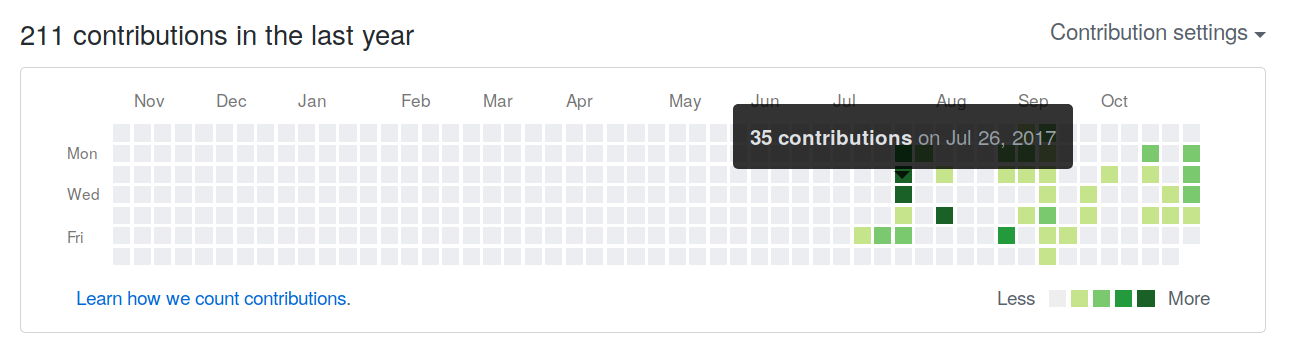
\includegraphics[width=\textwidth]{ResultadosyDiscusion/Figs/contributions.png}
\caption{Calendario de actividad y contribuciones de este trabajo al proyecto \pgland{} (\textit{heatmap calendar}). \label{fig:contrib}}
\end{center}
\end{figure}

Siguiendo con la figura \ref{fig:contrib}, los colores más intensos indican días de una mayor actividad, siendo el día 26 de julio el día en el que más aportaciones se realizó. Un número tan grande de aportaciones es normal en la puesta en marcha de un proyecto de este tipo y en particular fue el día en el que se incorporaban sentencias SQL que habían sido testeadas en días anteriores. Según la complejidad de las métricas o las funciones a desarrollar, hay días con una menor actividad y, en aquellos casos más problemáticos, también hay días en los que los desarrollos los hacían otros miembros del equipo y había tiempo de preparar conjuntos de datos de ejemplo, preparar documentación o trabajar en la redacción del presente trabajo.

En total se ha contribuido al proyecto con 211 aportaciones, que posteriormente han sido aceptadas en la mayoría de los casos. El proyecto oficial únicamente muestra 209 contribuciones, pero ambas cifras no están directamente relacionadas. Hay que tener en cuenta que las acciones de \textit{pull request} explicadas en la figura \ref{fig:pullrequest} de la metodología suelen empaquetar varias actualizaciones o \textit{commits} que en el repositorio oficial aparecen como una única aportación. GitHub permite analizar el trabajo y la contribución de cada miembro del equipo de un modo muy minucioso.

El control de versiones sirve para recuperar un punto de trabajo anterior o también para supervisar cómo se ha ido desarrollando un trabajo. Aproximadamente, a partir de la figura \ref{fig:contrib} y otras similares es posible reconstruir las fases principales en que se desarrolló este trabajo. En julio se hizo una revisión bibliográfica y se aprendió a utilizar las herramientas vistas en la metodogía. A finales de julio se seleccionaron y se crearon consultas SQL para calcular la mayoría de las métricas. En agosto se creó un conjunto de datos de ejemplo y se validaron los resultados de cada consulta. En septiembre se convirtieron las consultas en funciones simples y, dado que no todas las métricas se podían implementar del mismo modo, en octubre se modificaron varias funciones para convertirlas en funciones de agregación. Finalmente, en noviembre se realizó el experimento computacional cuyos resultados se muestra en la sección \ref{sec:caso_uso}.

En el diagrama de red de GitHub (ver figura \ref{fig:network}) se puede visualizar el trabajo colaborativo desarrollado desde el principio hasta la realización de la experiencia computacional presentada en este trabajo. Se trata de un diagrama dinámico en el cual se puede consultar el contenido de cada contribución, ya sea la creación de nuevas funciones o cambios. En la figura \ref{fig:network} se pueden ver varios \textit{commits} por parte de distintos colaboradores, una operación de \textit{pull upstream}, cuatro operaciones \textit{push} y una serie de contribuciones propias que aún no habían sido aceptadas por el equipo del proyecto SIOSE-INNOVA. Los colores de las líneas ayudan a interpretar mejor este tipo de diagramas:

\begin{itemize}
\item La línea negra muestra los \textit{commits} integrados en el repositorio oficial.
\item Las líneas verdes y azules se refieren a aportaciones de este trabajo que finalmente fueron aceptadas por el equipo del SIOSE-INNOVA.
\item La línea morada hace referencia a las últimas funciones creadas, pendientes de aceptación al término de este trabajo.
\end{itemize}

\begin{figure}
\begin{center}
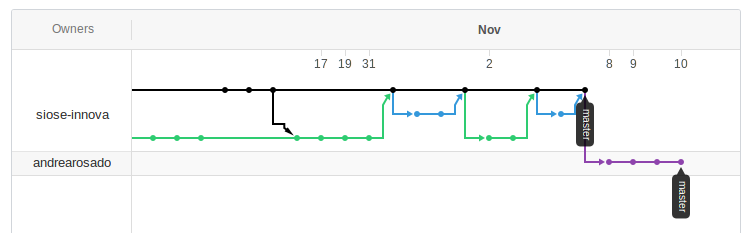
\includegraphics[width=\textwidth]{ResultadosyDiscusion/Figs/network.png}
\caption{Diagrama de red de GitHub.  \label{fig:network}}
\end{center}
\end{figure}

En cuanto a los resultados concretos de este trabajo, se han desarrollado 25 funciones sobre PostgreSQL/PostGIS que calculan métricas del paisaje de distintos tipos (a nivel de polígono, categorías y paisaje). Todas las funciones se han creado por duplicado (\textit{funciones sobrecargadas}) para trabajar con sistemas de coordenadas planas y con coordenadas geográficas. Esta decisión tiene que ver con que en bases de datos tan voluminosas como la del SIOSE, en ocasiones será necesario realizar cálculos con polígonos que se encuentren muy distantes, llegando incluso a representarse en usos o sistemas de referencia espacial distintos. El uso de coordenadas esféricas permite trabajar con una geodatabase sin preocuparse de este tipo de problemas, pero a cambio de poder utilizar un número menor de funciones de PostGIS. No obstante, resulta que todas las métricas seleccionadas a partir de la documentación de FRAGSTATS han podido ser calculadas partiendo del tipo \textit{geography} de PostGIS. Esto hace que las operaciones con el SIOSE resulten más sencillas si no es necesario dividir la base de datos por usos o comunidades autónomas.

A parte de todas las funciones de cada una de las métricas seleccionadas, se han desarrollado dos funciones tipo ya que así permite obtener los resultados estructurados, es decir, que el valor obtenido vaya acompañado de su etiqueta a la métrica que corresponde, a la categoría a la que pertenece y de las unidades correspondientes. Además esto a facilitado el trabajo a la hora de simplificar las funciones de tipo agregado ya que a cada métrica y unidad de valor le corresponde un identificador único. Por otra parte, hay que tener en cuenta que también se ha tenido que desarrollar unas consultas test SQL para realizar el experimento y obtener resultados representativos que quedan expuestos en la sección \ref{sec:caso_uso} y la función final la cual nos permite obtener todos los resultados en una sola secuencia (ver la sección \ref{sec:exp}). 

En la tabla \ref{tab:metrics-ext} se listan todas las métricas del paisaje implementadas en la extensión. Los colores indican si la métrica se ha podido desarrollar como una función SQL simple o si por el contrario ha sido necesario crear una función de agregación (combinación de varias funciones). 

% Please add the following required packages to your document preamble:
% \usepackage{booktabs}
% \usepackage[table,xcdraw]{xcolor}
% If you use beamer only pass "xcolor=table" option, i.e. \documentclass[xcolor=table]{beamer}
\begin{table}[]
\centering
\caption{Listado de las métricas de paisaje disponibles en la extensión, según su nivel de complejidad y si han sido aceptadas en el repositorio oficial.}
\label{tab:metrics-ext}
\begin{tabular}{@{}lcccl@{}}
\toprule
\textbf{Métrica} & \textbf{Manual/QGIS} & \textbf{Consulta SQL} & \textbf{\pgland{}} \\ \midrule
\rowcolor[HTML]{F9F9D2}
AREA                    & \bullet       & \bullet      & \bullet            \\
\rowcolor[HTML]{F9F9D2}
PERIM                   & \bullet       & \bullet      & \bullet            \\
\rowcolor[HTML]{F9F9D2}
PARA                    & \bullet       & \bullet      & \bullet            \\
\rowcolor[HTML]{F9F9D2}
SHAPE                   & \bullet       & \bullet      & \bullet            \\
\rowcolor[HTML]{F9F9D2}
CORE                    & \bullet       & \bullet      & \bullet            \\
\rowcolor[HTML]{F9F9D2}
NCORE                   & \bullet       & \bullet      & \bullet            \\
\rowcolor[HTML]{F9F9D2}
CAI                     & \bullet       & \bullet      & \bullet            \\
\rowcolor[HTML]{F9F9D2}
ENN                     & \circ         & \bullet      & \circ              \\
\rowcolor[HTML]{DBF1DA}
CA                      & \bullet       & \bullet      & \bullet            \\
\rowcolor[HTML]{DBF1DA}
PLAND                   & \bullet       & \bullet      & \bullet            \\
\rowcolor[HTML]{DBF1DA}
TE                      & \bullet       & \bullet      & \circ              \\
\rowcolor[HTML]{DBF1DA}
ED                      & \bullet       & \bullet      & \circ              \\
\rowcolor[HTML]{DBF1DA}
TCA                     & \bullet       & \bullet      & \circ              \\
\rowcolor[HTML]{DBF1DA}
CPLAND                  & \bullet       & \bullet      & \circ              \\
\rowcolor[HTML]{DBF1DA}
NP                      & \bullet       & \bullet      & \circ              \\
\rowcolor[HTML]{DBF1DA}
PD                      & \bullet       & \bullet      & \circ              \\
\rowcolor[HTML]{DBF1DA}
TA                      & \bullet       & \bullet      & \bullet            \\
\rowcolor[HTML]{DBF1DA}
TE                      & \bullet       & \bullet      & \bullet            \\
\rowcolor[HTML]{DBF1DA}
ED                      & \bullet       & \bullet      & \bullet            \\
\rowcolor[HTML]{DBF1DA}
NP                      & \bullet       & \bullet      & \bullet            \\
\rowcolor[HTML]{DBF1DA}
PD                      & \bullet       & \bullet      & \bullet            \\
\rowcolor[HTML]{DBF1DA}
PR                      & \bullet       & \bullet      & \circ              \\
\rowcolor[HTML]{DBF1DA}
PRD                     & \bullet       & \bullet      & \circ              \\
\rowcolor[HTML]{DBF1DA}
SHDI                    & \bullet       & \bullet      & \circ              \\
\rowcolor[HTML]{DBF1DA}
SHIDI                   & \bullet       & \bullet      & \circ  
\\ \midrule           
                        &                      &       & 
\\
\cellcolor[HTML]{F9F9D2}Función simple &       &       & 
\\
\cellcolor[HTML]{DBF1DA}Función agreg.&   &       & 
\\
\bullet \ Aceptada              &         &       & 
\\
\circ \ Pendiente               &         &       & 
\\
\end{tabular}
\end{table}

En esta tabla de resumen también se puede ver que prácticamente todas las consultas se podían calcular manualmente (independientemente de la dificultad) salvo la distancia euclídea al vecino más próximo (ENN; Euclidean Nearest Neighbour Distance). Esta métrica implica numerosos cálculos de distancia entre polígonos, el uso de índices espaciales y la aplicación de una serie de filtros. Evidentemente, el cálculo del ENN resultaría muy trabajoso si no se utiliza ningún lenguaje de programación. La consulta SQL para el ENN se realizó de un modo más o menos sencillo. Sin embargo, su implementación como función SQL de agregación está aún siendo revisada por el equipo del SIOSE-INNOVA.

Las métricas marcadas como pendientes de aceptación en la tabla \ref{tab:metrics-ext} devuelven el resultado correcto con el paisaje de ejemplo descrito en este trabajo, por lo que \textbf{es de esperar que pronto pasen a formar parte del repositorio oficial de \pgland{}}.

En relación con los objetivos de este trabajo y del proyecto SIOSE-INNOVA, resulta muy significativo el modo en que se han simplificado todas las tareas de desarrollo y cálculo de las métricas del paisaje. Los miembros del equipo de trabajo pueden disponer, en cuestión de minutos, de una versión actualizada de la extensión \pgland{} con los últimos cambios realizados por otro compañero. Esta versión actualizada se obtiene mediante la ejecución de un sencillo comando (\textit{docker-compose up}) y viene acompañada de todo el software necesario para trabajar, incluyendo las mismas opciones de configuración utilizadas por todo el equipo. Igualmente, resulta también sencillo trabajar en laboratorio desde un servidor o desde un portatil en casa. Más aún, la tecnología utilizada funciona en los sistemas operativos más utilizados (Linux GNU, Windows o Mac). 

Los usuarios finales de \pgland{} o de la base de datos del SIOSE, también verán facilitado su trabajo, ya que las 25 métricas implementadas simplifican en gran medida las consultas necesarias para realizar este tipo de análisis. Por ejemplo, una métrica en apariencia tan sencilla como Total Core Area (TCA) pasa a calcularse en una única línea frente a las más de 20 líneas que serían necesarias en SQL (ver ejemplos de código \ref{lst:tca2} y \ref{lst:tca3}).

Así mismo, la extensión \pgland{} está 

\section{Caso de uso sobre el SIOSE-2011 \label{sec:caso_uso}}

Los objetivos de este trabajo incluyen la realización de una experiencia computacional sobre una geodatabase voluminosa. Se trata de poner a prueba la extensión \pgland{} (y las tecnologías sobre las que trabaja) para valorar si sería posible ofrecer un servicio de consultas sobre el SIOSE similar al descrito en la figura \ref{fig:visorweb} de este trabajo. Este caso de uso se ha descrito en detalle en el capítulo \ref{chap:metod}. El experimento completo se ha lanzado a partir de una única consulta SQL (ver ejemplo de código \ref{list:runtests}).

En este experimento se calculan las métricas \textit{Patch Area (AREA)}, \textit{Total (Class) Area (CA)} y \textit{Total Area (TCA)} a diferentes escalas de referencia y se recuperan sus resultados junto con los tiempos de cálculo. Los resultados de este experimento pueden visualizarse en las figuras incluidas en esta sección y en el Anexo \ref{anex:results}. En estas figuras se ven las dos zonas cuya estructura se quiere comparar (zonas de Alicante y Zaragoza), cada celda representada se correspondería con una operación de \textit{zoom} o desplazamiento de un usuario dentro de un visor web.

En estas figuras, los resultados están representados mediante el método de clasificación de desviación estándar que muestra los valores medios en rangos iguales; aquellos valores que se encuentren más alejados de la media están representandos por distinto colores, naranja para aquellas celdas que presentan un valor menor, y morado para aquellas celdas con un valor mayor. En todas las figuras también es posible ver el tiempo total de cálculo para cada zona, es decir para varias operaciones de cálculo.

En la figura \ref{fig:p_25}, se muestran todos los cálculos de la métrica Patch Area (AREA), de modo que se pueden comparar las dos zonas de estudio a escala 1:25.000. Este ejemplo presenta una estructura similar entre las dos zonas. Sin embargo, al noreste de la zona de Zaragoza se ve una peculiaridad. Si se observa con más detalle, la celda de color morado más oscuro presenta unos valores significativamente por encima de la media. Esto se debe a que la intersección de la celda con los polígonos del SIOSE afecta a 6 polígonos de una considerable extensión (ver figura \ref{fig:ejemplo}). Por lo tanto, es lógico que el cálculo realizado devuelva un valor tan elevado. De este modo, el cálculo de AREA a nivel de polígono puede utilizarse para interpretar la estructura del paisaje de un modo rápido. Allí donde se den anomalías que distingan un paisaje del otro estará relacionado con la presencia de polígonos relativamente extensos.

\begin{figure}
\begin{center}
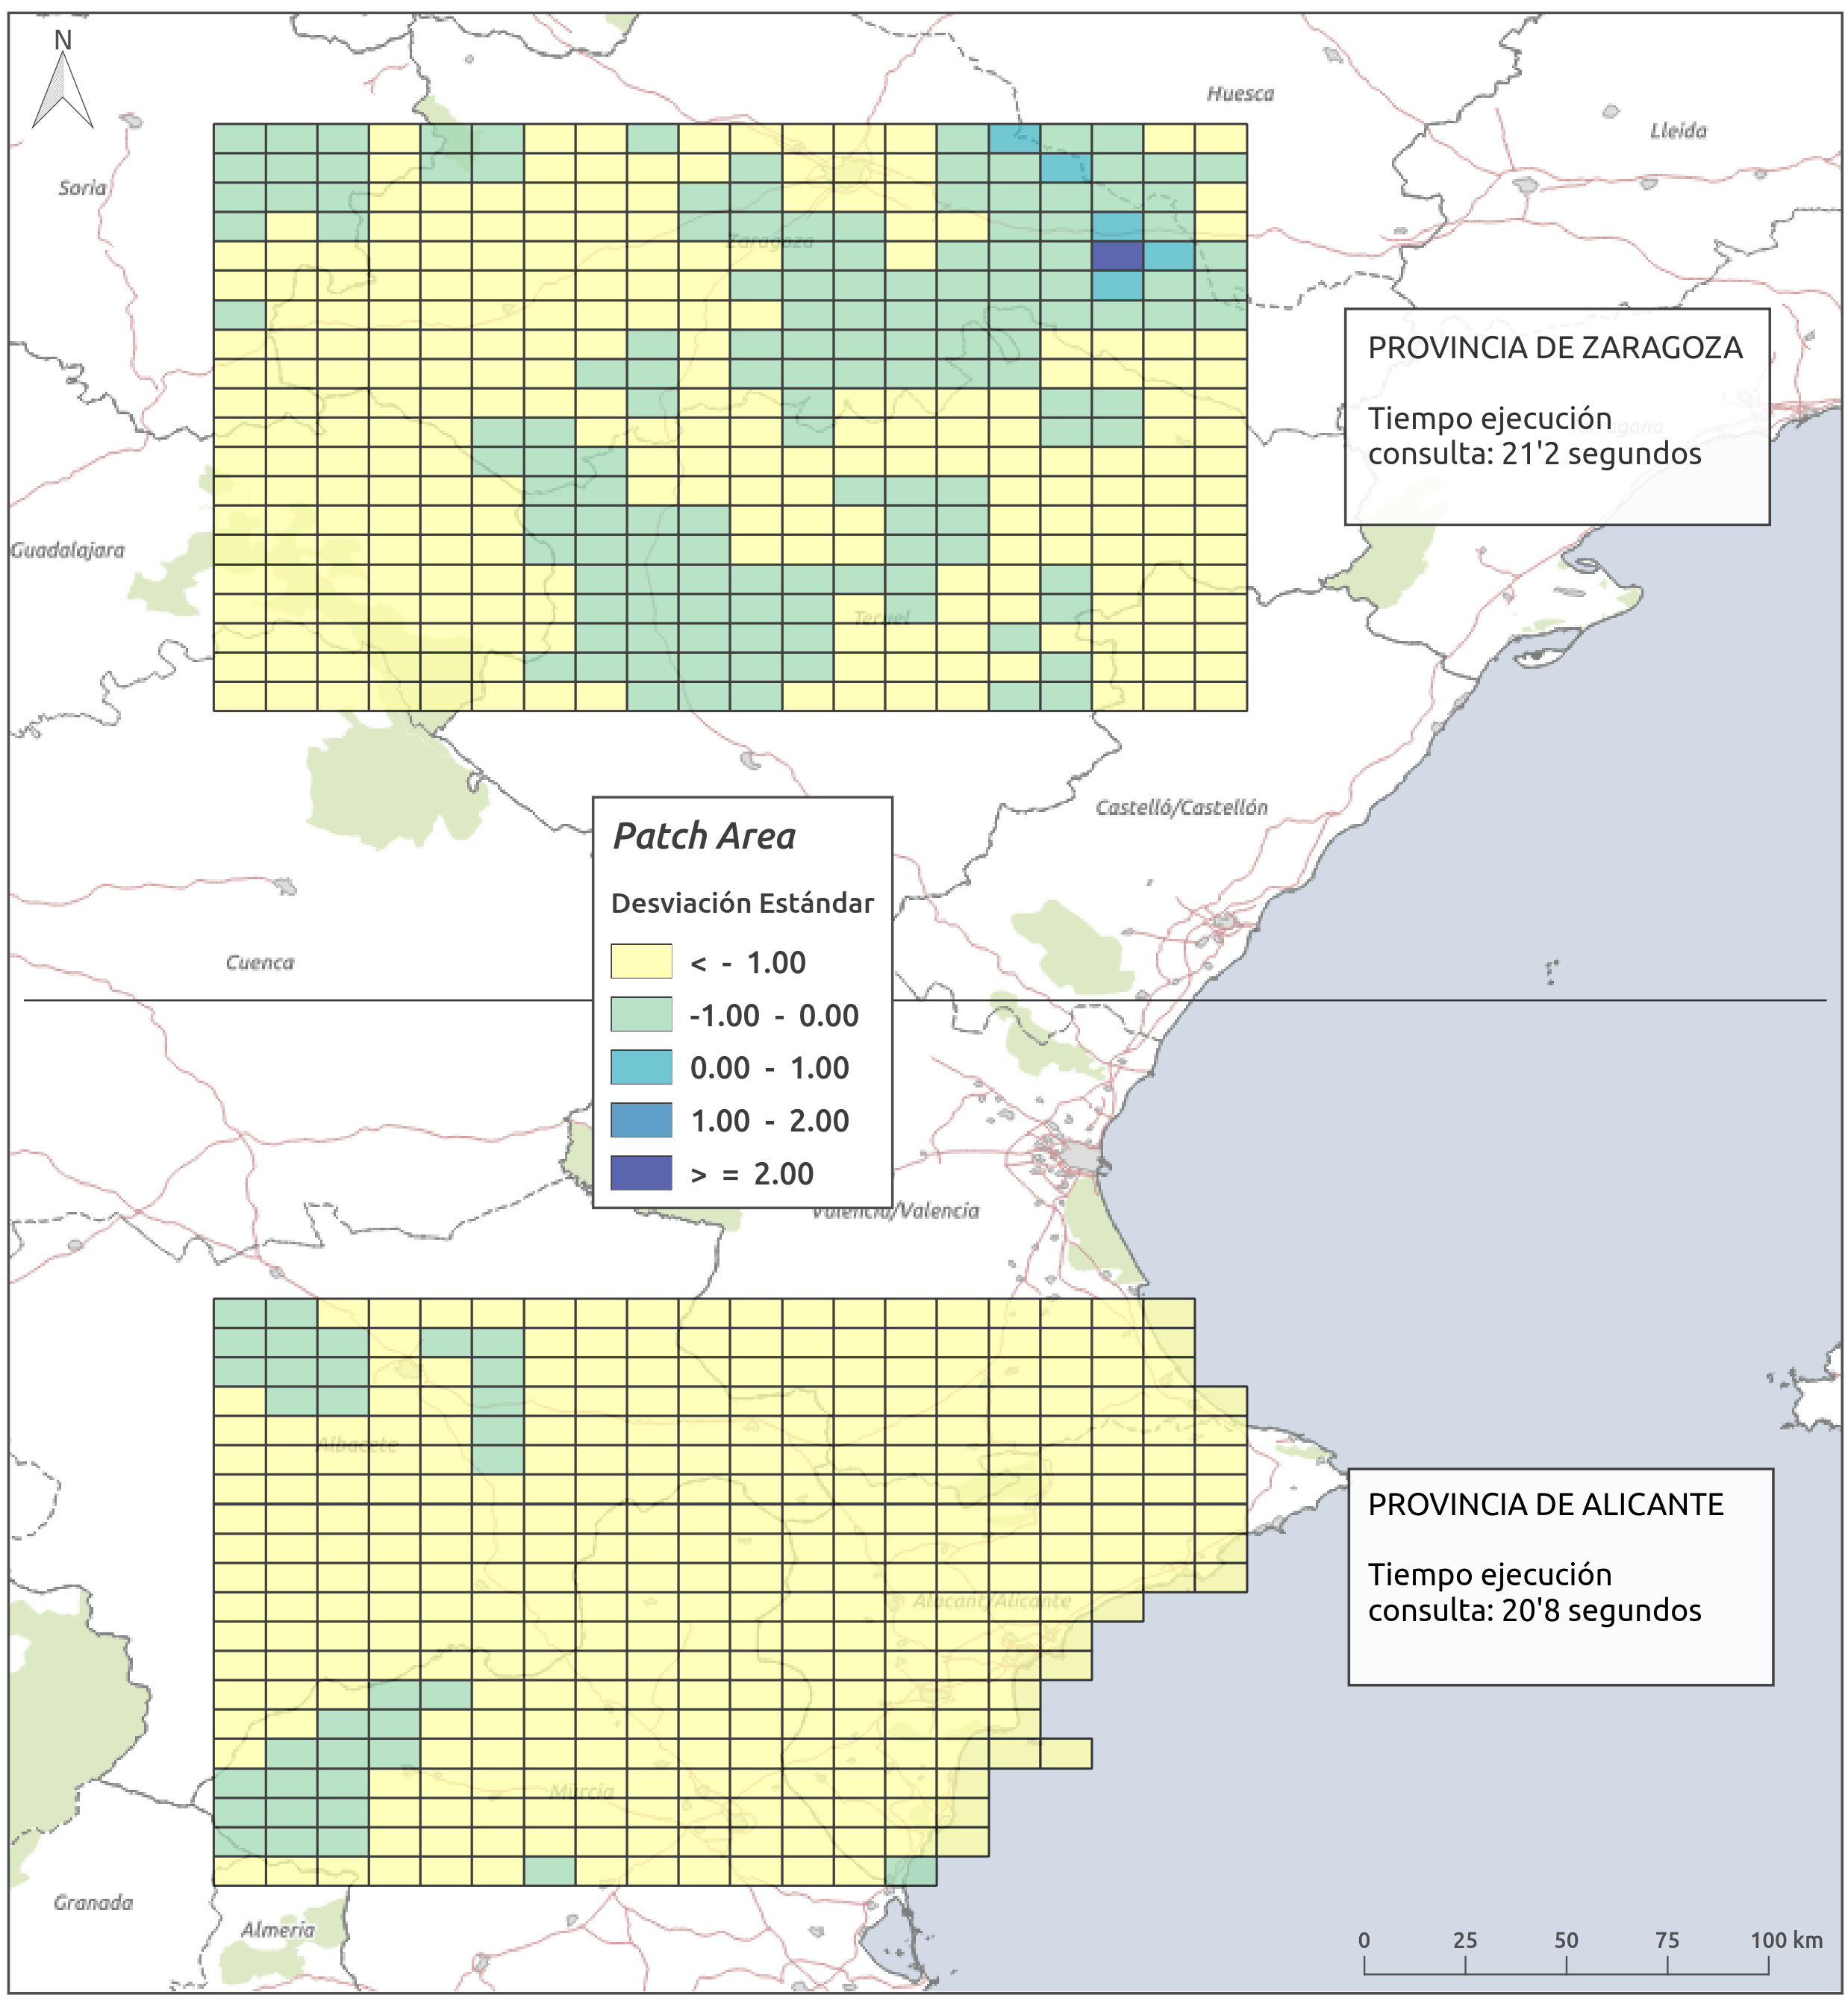
\includegraphics[width=\textwidth]{ResultadosyDiscusion/Figs/Results/p_25.png}
\caption{Resultado de la métrica AREA en la zona de Alicante y Zaragoza a partir del grid 1:25.000. \label{fig:p_25}}
\end{center}
\end{figure}

\begin{figure}
\begin{center}
\includegraphics[width=\textwidth]{ResultadosyDiscusion/Figs/ejemplo.png}
\caption{Ejemplo de anomalía en la zona de Zaragoza. \label{fig:ejemplo}}
\end{center}
\end{figure}

Por otro lado, se ha querido mostrar el resultado del cálculo del área a nivel de categoría. Para ello se han seleccionado algunas que pertenezcan a la clase de forestal como: prados (290), pastizal (300), frondosas caducifolias (312), frondosas perennifolias (313), coníferas (316) y matorral (320). Cabe mencionar que la elaboración de esta clasificación de ocupación del suelo queda explicada en el capítulo \ref{chap:metod}. En la figura \ref{fig:c_25}, calculada la métrica Total (Class) Area (CA), a raíz de la selección de las categorías anteriores se puede apreciar aproximadamente la disposición del relieve donde en las zonas más interiores se encuentran los polígonos con mayor área.

A parte de la representación visual de los resultados, otro aspecto importante es el tiempo de ejecución de todas las consultas SQL que se han realizado para cada una de las zonas con sus respectivas métricas y grids. A modo de síntesis, la métrica a nivel de paisaje presenta un tiempo menor respecto a las otras como también es el caso de la zona de Zaragoza respecto a la zona de Alicante. Esto puede ser motivo a que alguna de las dos zonas tenga que ejecutar la consulta para un número menor de polígonos o según la complejidad que presente el cálculo de la métrica de paisaje. Todo los resultados y tiempos se encuentran en el anexo \ref{anex:results}.



\begin{figure}
\begin{center}
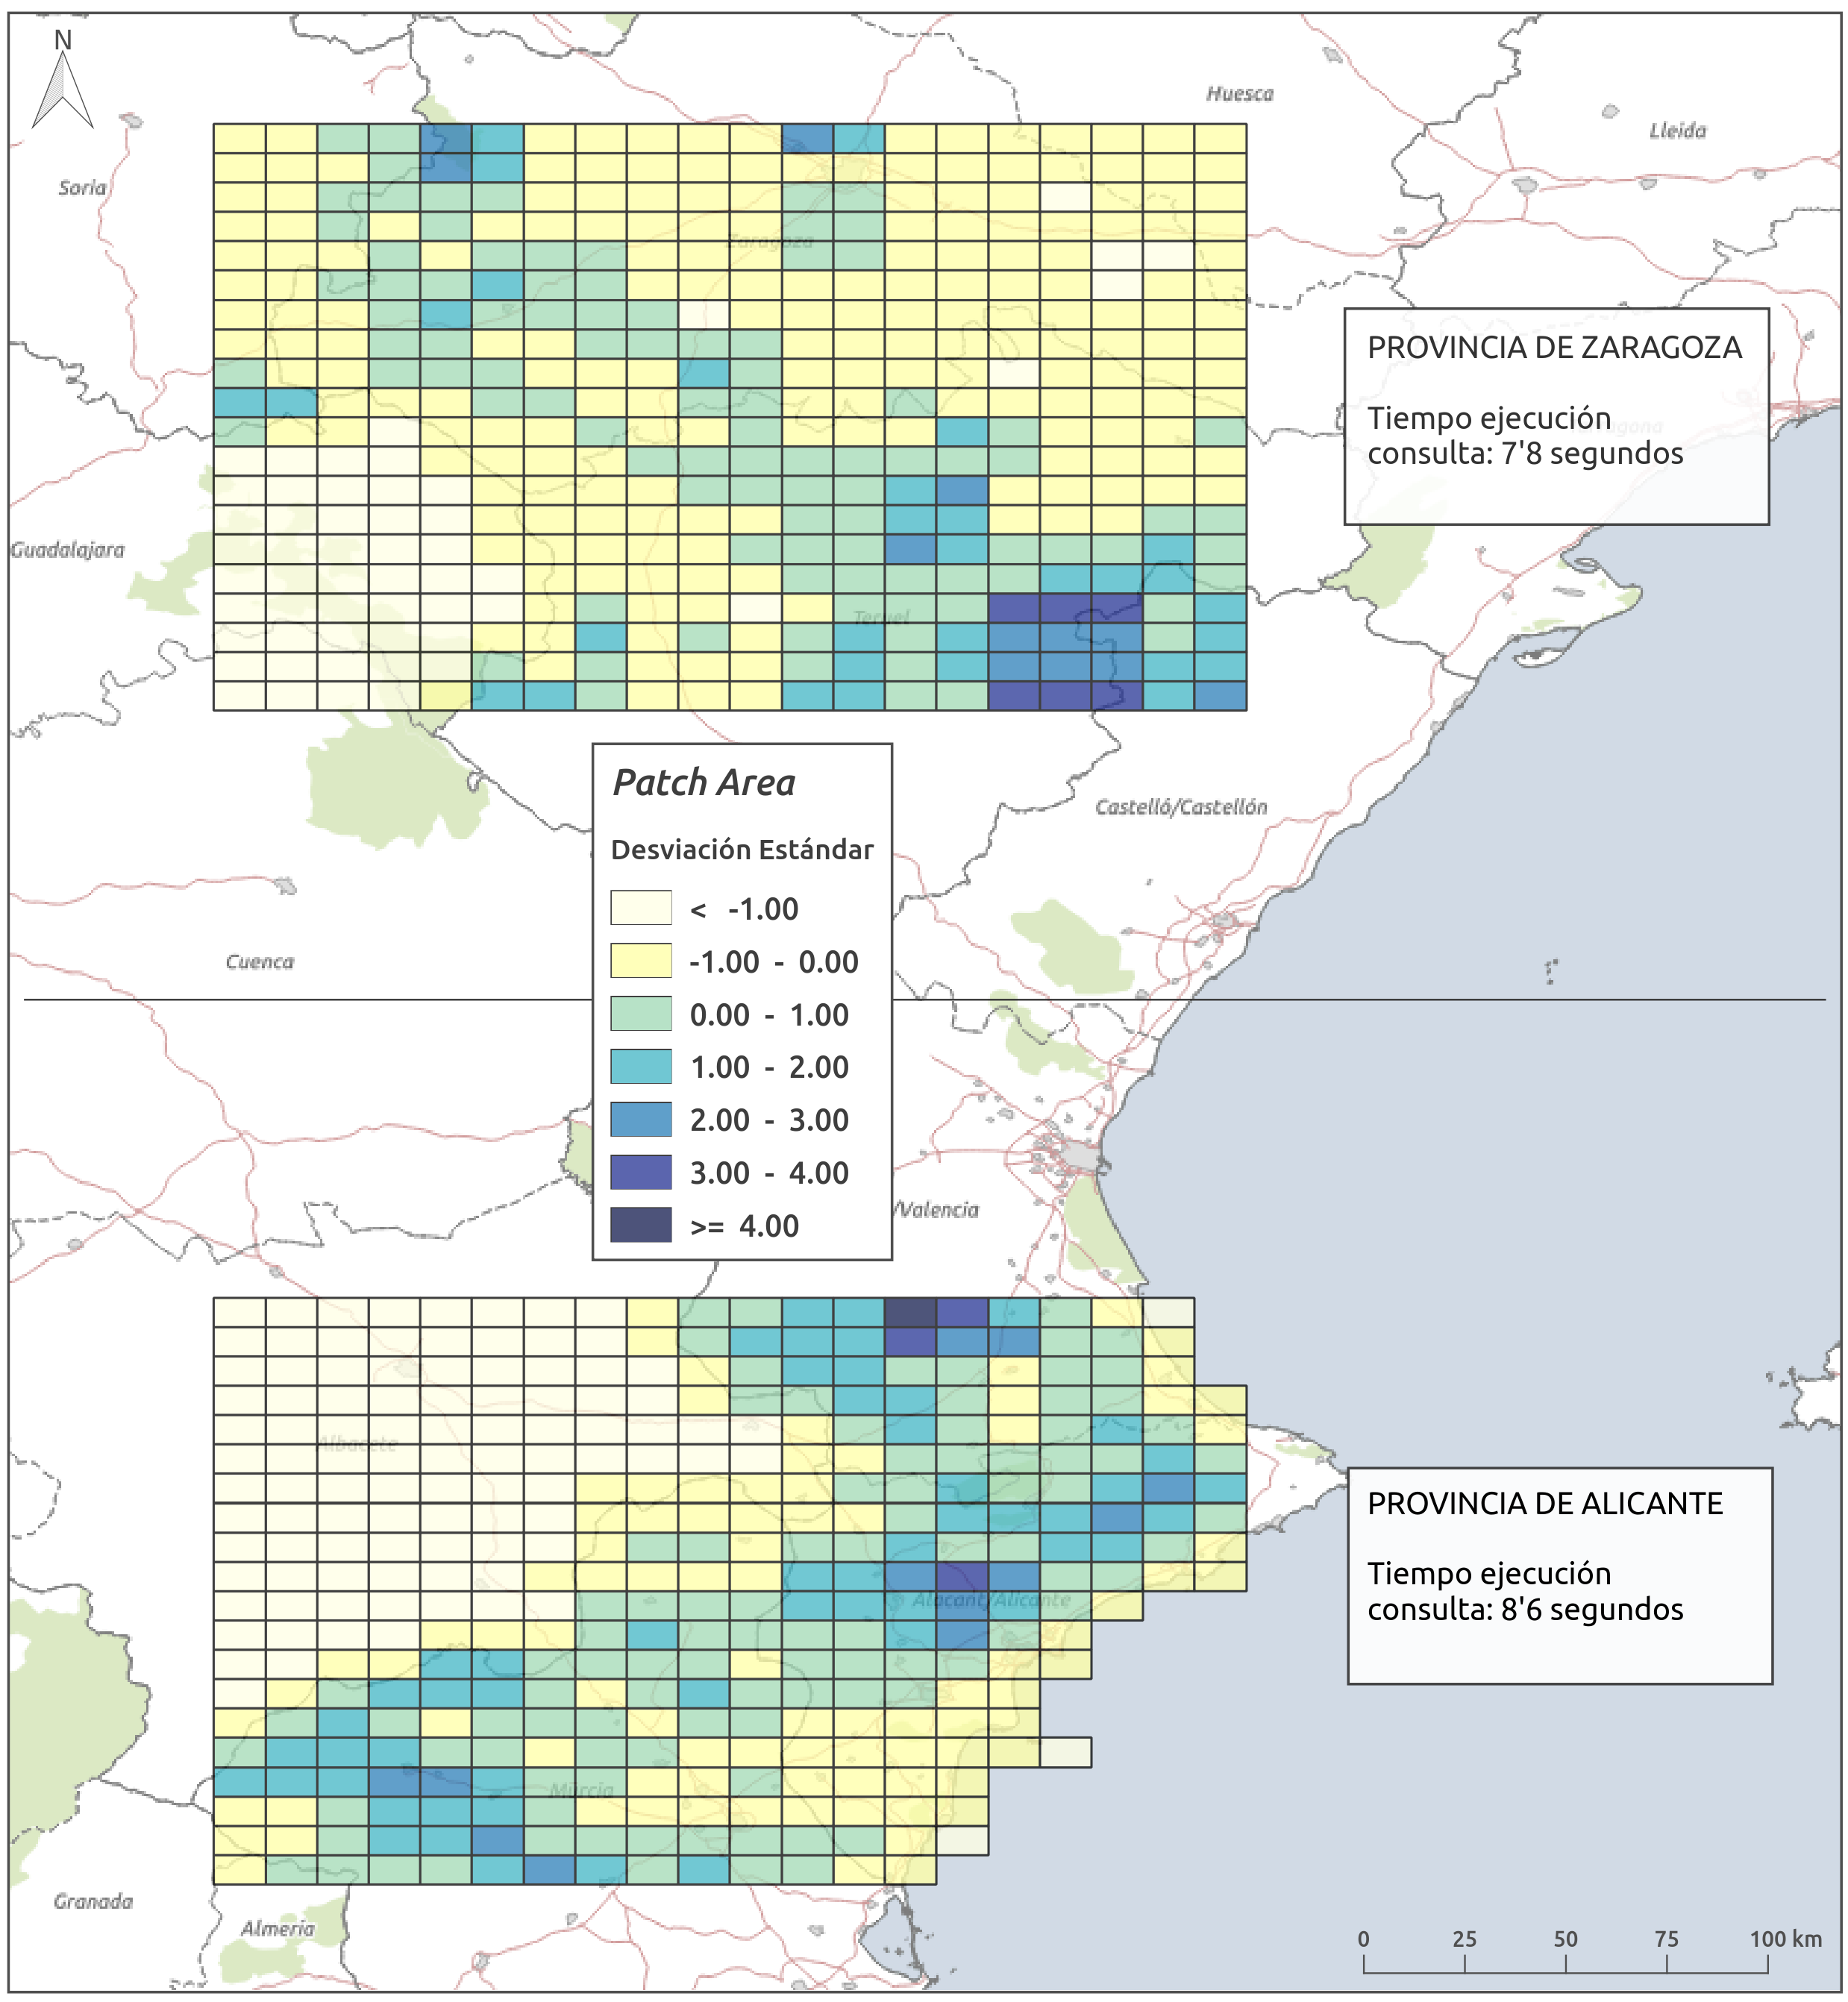
\includegraphics[width=\textwidth]{ResultadosyDiscusion/Figs/Results/c_25.png}
\caption{Resultado de la métrica CA en la zona de Alicante y Zaragoza a partir del grid 1:25.000. \label{fig:c_25}}
\end{center}
\end{figure}